% CONCLUSIONS
\chapter*{Synthèse et perspectives}
\markboth{Conclusions et perspectives}{}
\addcontentsline{toc}{chapter}{Conclusions et perspectives}
\newpage

schéma conceptuel ? Modèles globaux (ORCHID, chloée)

\section{Bilan du bilan (de C) ?}

Flux fort

sensibilité param forte

Modèles multi annuel et prise en compte de la végétation

Quid des variations journalières dans un bilan annuel ? (Figure~\ref{fig:RE1_vs_JN})

\begin{figure}
\centering
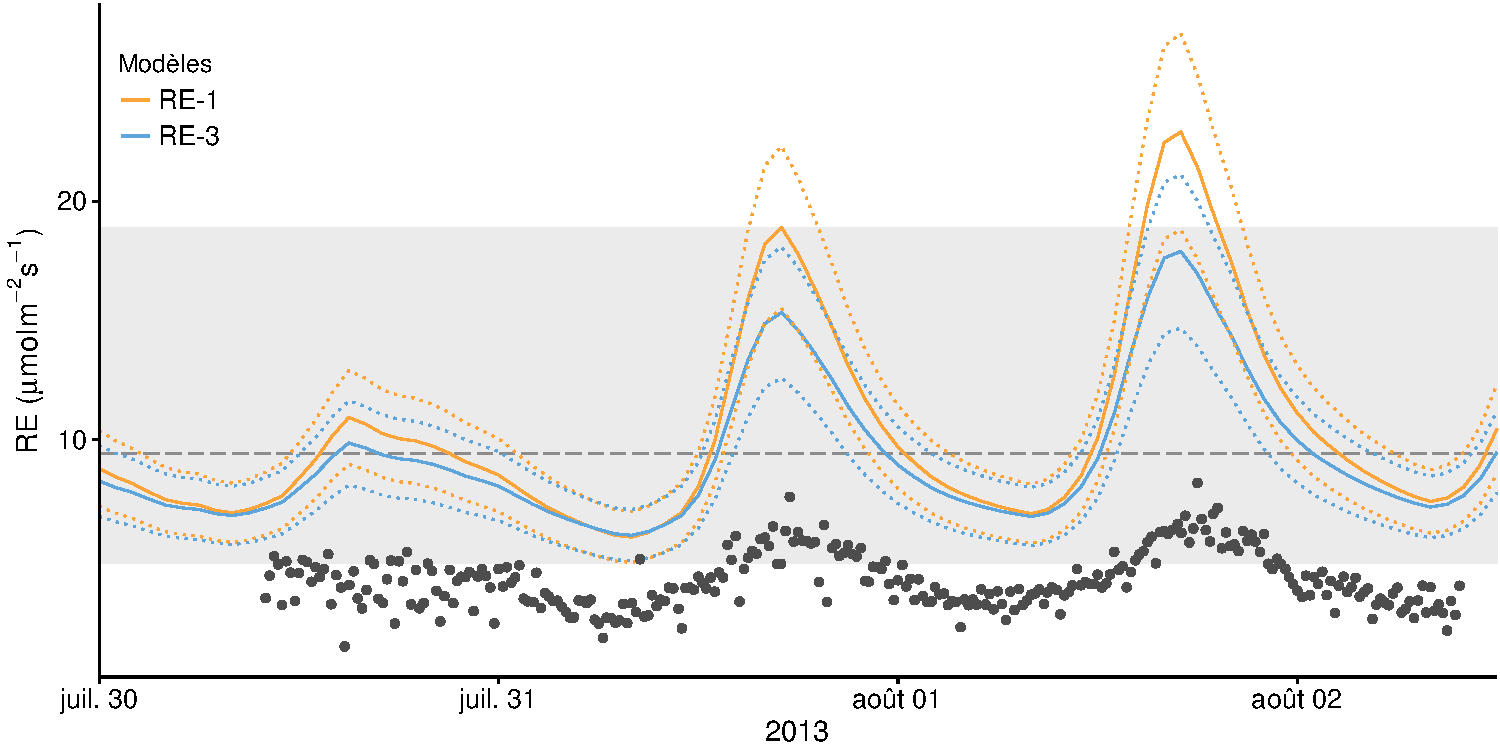
\includegraphics[width=\textwidth]{conclusions/RE1_vs_JN}
\caption{Comparaison entre les valeurs estimées par le modèle RE-1 et les mesures faites à haute fréquence sur le site du 30 juillet au 2 août 2013}
\label{fig:RE1_vs_JN}
\end{figure}


Les prendre en compte améliorerait-il les modèles

modèles globaux ?
\textbf{limitations deséquations :}
Plus généralement, la majorité des tourbières sont sous la neige une partie de l'année, ce qui n'arrive que rarement sur la tourbière de La Guette et une partie possède également des zones d'eau libre, qui n'existent pas sur ce site.

modèles globaux et profondeur de tourbe

\section{Résilience de la tourbe par rapport aux 2 années sèches qui précèdent le BdC}
(lien chap 3 et 4)

\section{Ouverture vers d'autre méthodes de mesures}
\begin{itemize}
\item chambre automatique (lien chap 5, et chap 3 ?)
\item tour eddy covariance (lien chap 5 et chap 3 ?)
\end{itemize}
